%===================================== CHAP 5 =================================

\chapter{System Architecture}

\section{Architecture Description}
The web portal can be divided into back end and front end (see fig. \ref{Architecture}).
\\On back end, Nginx is used to serve the static files and media requested by the client. All other requests are routed to a server hosted by Django. This server is responsible for routing to sub-pages, authentication and rendering of templates. The SQLite database is also running on this server, providing efficient data flow. The data in the database can only be accessed through the server, thus making it secure.

On front end, the client receives files from the server to be displayed in a browser. Some of the files contains components created using the React library. These components takes user input, exchange data with the server and display the new information, offering a dynamic behaviour in the web portal.

\begin{figure}[ht]
\centering
    \includegraphics[width=1\textwidth]{fig/Architecture}
\caption{Architecture}
\label{Architecture}
\end{figure}

\section{Back End}
The back end was written in Python (see \ref{python}) using the Django framework (see \ref{django}), and is the application's logical layer. It communicates with the front end layers, validates information that comes from clients and serves the outgoing information. Database restrictions are also managed by this layer. All information that flows through the database is created, validated and updated at this stage. 


\subsection{Database Structure}
The database is structured in four different tables; User, User Profile, Activity and Organizations(Providers). These four tables are combined together by three different relational tables, and one single relation between the User table and the User Profile table. The relational tables are Participated In, Employed In and Hosts (see fig. \ref{Database_Figure}).

The User table is a predefined table created by the Django framework (see \ref{django}). The group chose to use this table to manage User identification, as it is a part of Django's security authentication. The customer also desired to divide the users into groups, such as a family. Due to this requirement, the group chose to create a User Profile table which is dependent on the User table. This allowed for customizing user profiles and creating user groups, without tampering with the authentication system. 

The rest of the database behaves like a relational database.

\begin{figure}[ht]
\centering
    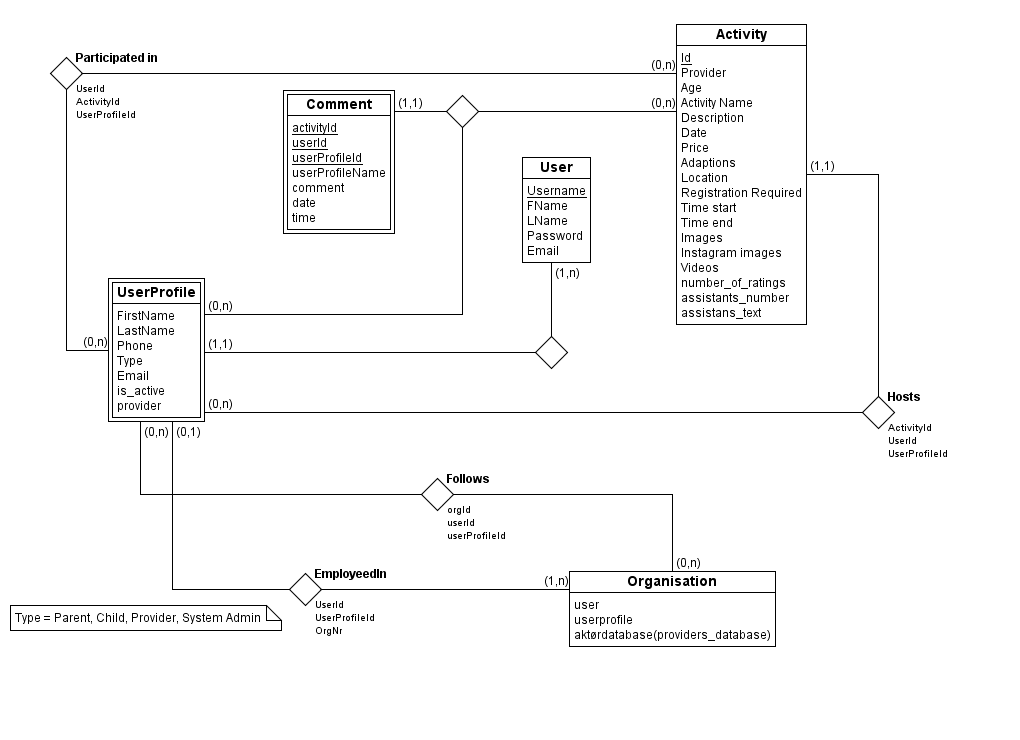
\includegraphics[width=0.90\textwidth]{fig/erDatabase}
\caption{Database structure}
\label{Database_Figure}
\end{figure}


\subsection{Access to Aktørbasen}
\label{Aktordatabasen}
One of the most essential requirements defined during the first meeting with the customer (see \ref{Customer input}), was the need for the web portal to interact with Trondheim Kommune Aktørbase. It was important that the leisure activity providers whom already have been registered in this database, could reuse their account or information. Furthermore, making it more appealing to start using the web portal.

Another aspect of the interaction with the Aktørbase, was the opportunity to extract registered leisure activities and leisure clubs, presenting this to users through the  web portal. This would allow the users to easily search for them, similar to a Google search. 

During the development process the group performed a focus group with the developers and project leader of Trondheim Kommune Aktørbase, to discuss the opportunities and later usage of the Aktørbase (see section \ref{focusGrouoProviders}).

Aktørbasen is still under development. During the meeting with their representatives the group made an suggestion that it should contain additional information, about leisure activities- and providers, in the future. This information should be available through an API, giving the web portal access to the information. Since this solution does not yet exist, the group created a program that queries the official interface of the Aktørbase,extracting the relevant information. This solution was used during development to show Trondheim kommune a possible usage of their database, and encourage future cooperation with skalvi.no. 

\section{Front End}
The front end was primarily written in HTML5, Javascript and CSS. To make the web portal dynamic and modern, additional frameworks and libraries like ReactJS, Redux, Bootstrap and Material Design Lite were utilized (see section \ref{frontEnd}). The HTML was written i Django Templates, which made it easy to create web pages with dynamic content. The front end is the application's visual layer, which is served by the logical layer. The visual layer also send information to the back end for validation.


\subsection{Data Flow}
The data flow figure (see fig. \ref{Data_Flow_Diagram}) was used to help the group get common understanding of the structure of the web portal. The figure shows where users can navigate to on the web portal given certain conditions. It shows that a user can always navigate to "Front Page" and "Activities Page", but must be logged in to be able to navigate to "Choose User Page" and "My Page". While being logged in the user can access "Create Activity Page", and "Edit Activity Page" if the user is hosting the specific activity. 

\begin{figure}[H]
\centering
    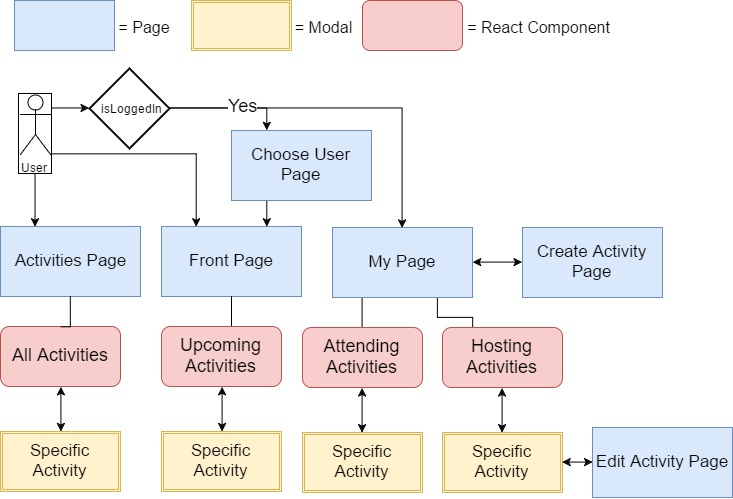
\includegraphics[width=\textwidth]{fig/dataFlow}
\caption{Data Flow}
\label{Data_Flow_Diagram}
\end{figure}

\subsection{Component Diagram}
The web portal contains five different pages (see fig. \ref{Component_Diagram}); Front Page, Activities Page, Providers Page, My Page and Create/Edit Activity Pages. Every page contains a navigation bar component for simple navigation. Only logged in users will have access to My page and Create Activity Page. Each activity component will become a modal if it is clicked, and users that created the activity will be able to edit.

\begin{figure}[H]
\centering
    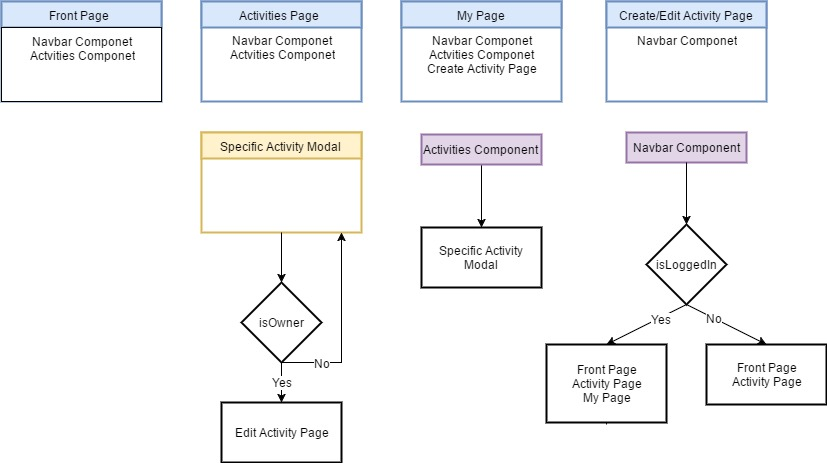
\includegraphics[width=\textwidth]{fig/Component_diagram}
\caption{Component Diagram}
\label{Component_Diagram}
\end{figure}

\subsection{Third Party Interfaces}
During the workshop with the users at the beginning of the project (see section \ref{WorkshopUserAndProviders}) and the weekly meetings with the customer (see section \ref{ss:customer_meetings}), solutions on how to create an unique and easy-to-use web portal were often suggested. Therefore, the use of third party interfaces, like Facebook's- and Instagram's Application Programming Interface (denoted as API), were considered and subsequently taken into use in the application. 

\subsubsection{Instagram API}
Instagram is a popular society, where users can upload and share images and videos. This content is available by using the API requests defined by Instagram.

An important concept to this project was taking benefit of all the information already available on the web. By connecting the web page to Instagram, users were allowed to use their already uploaded images when editing or creating an event.

\subsubsection{Facebook API}
During the workshop with the potential users of www.skalvi.no, the desire of being able to log in with Facebook was mentioned.

The customer emphasized that many providers use Facebook to display the activities they offer. Thus, it was requested to provide the opportunity to create activities based on existing Facebook events.  

Based on these requests, a connection to Facebook's own API was established. This allowed users and providers to securely log in to the portal, and retrieve events from Facebook. When a user logs in for the first time, access public profile information and user events must be accepted. 

\subsubsection{Log In}
During a weekly meeting with the customer, it was requested a modern way for families to log in. Inspiration from the Netflix log in solution was suggested, where families can log in with one username and password.

Therefore, registration of profiles using one specific main user was implemented. When the main user is logged in, it is possible to select which profile the user wants to use. It is also possible to change user profile at any time.

\section{Graphical User Interface}
The graphical user interface (denoted as GUI) was created in two phases. The first was to create a simple paper prototype and the second phase was to develop the user interface using the paper prototype as a template.

\subsection{Paper Prototype} \label{ss:paper_prototype}
The group designed the paper prototype in sprint 0 (see section \ref{sprint0}) as a first design draft of the application. See images of the prototype in Appendix \ref{paper_prototype}. This was a helpful asset for the group, as it created a common understanding of what was expected to be developed.

The paper prototype was presented to the costumer at the end of the sprint, the group explained the draft and the intended functionality that was to be developed. This created a common ground for the group and the costumer, ensuring the groups interpretation of the task was correct.  

\subsection{User Interface}
The design of the final product (see fig \ref{Front Page} and \ref{Modal}) was highly inspired by the paper prototype, as it had been created together as a group and further approved by the customer. 

The group aimed to design the web portal following the universal design principles (see section \ref{universalDesign}). This was considered essential due to the fact that the web portals user base are children with disabilities and disadvantages. This is reflected in how the group decided to manage focus marketing, and especially the use of colors to provide an better overview as well as hovering effects. Furthermore, the choice of supporting a dynamic search for activities and providers presented in an alphabetic list aimed to provide an easy search function for the users. 

The user interface is based on proverbial design principles; it uses symbols that users may have previously experienced on other sites, and can therefore use already acquired knowledge while using the web portal.  

\begin{figure}[H]
\centering
    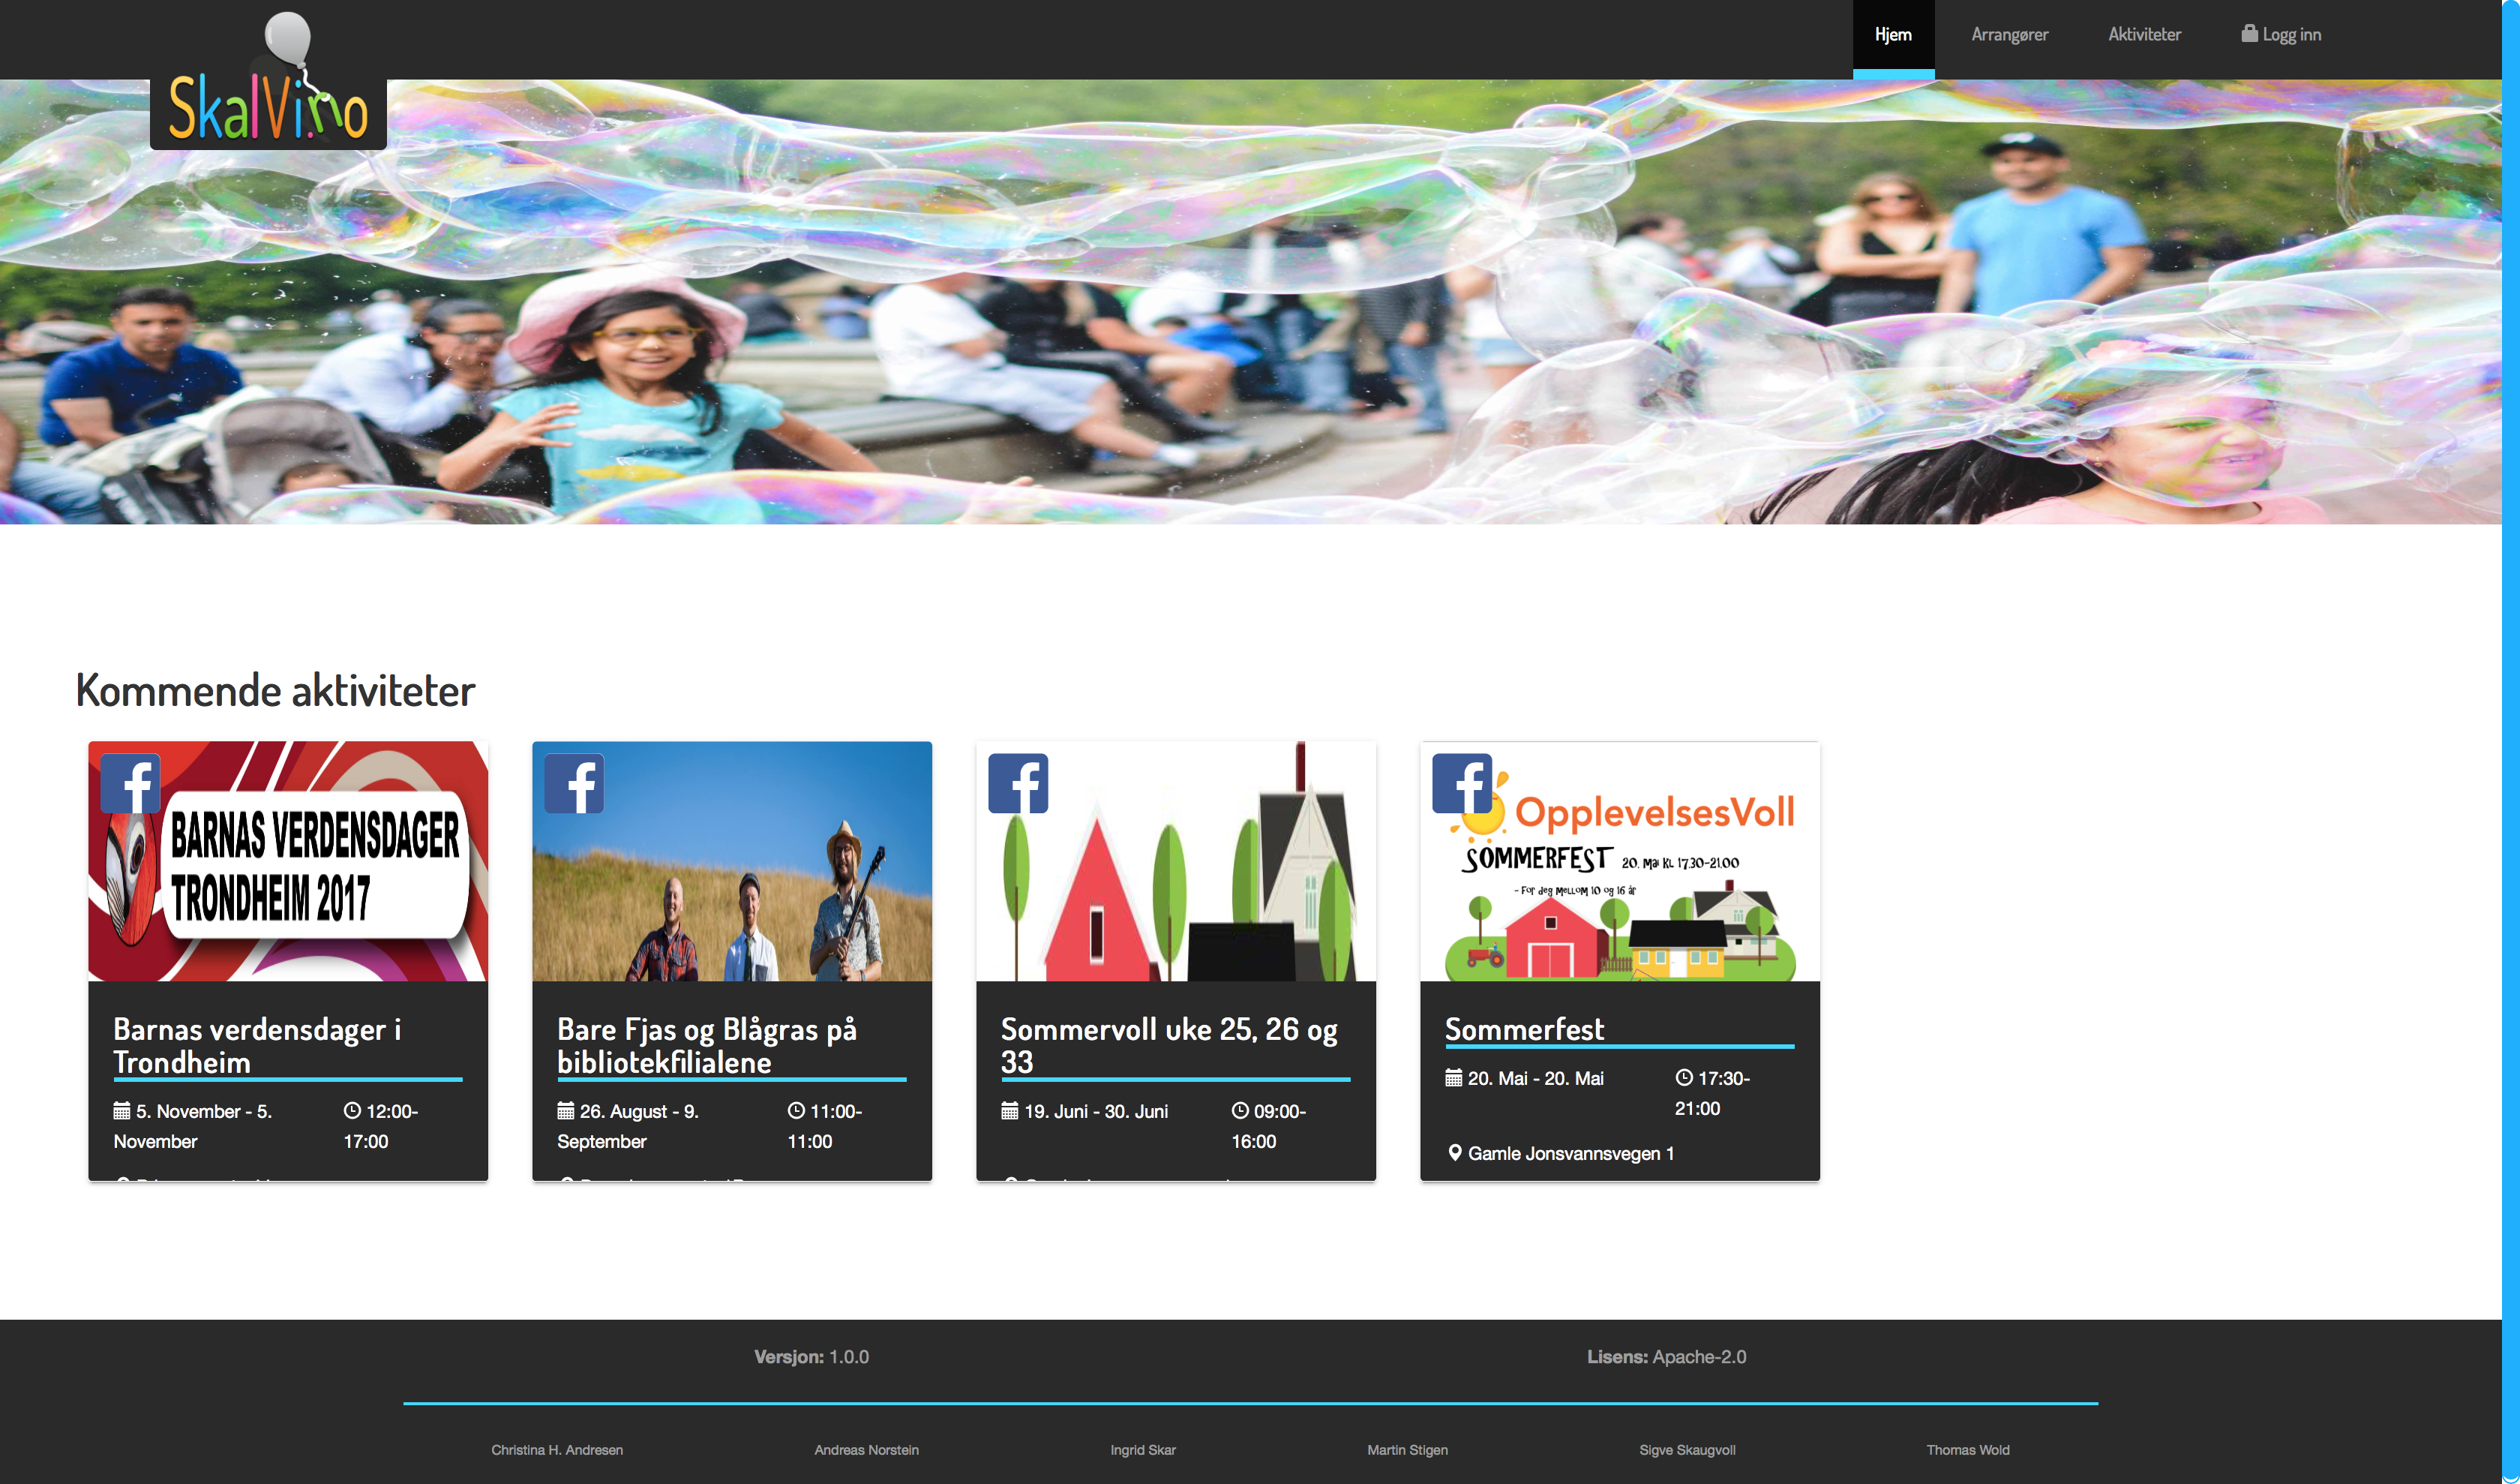
\includegraphics[width=\textwidth]{fig/frontpage.png}
\caption{User Interface - front page}
\label{Front Page}
\end{figure}

\begin{figure}[H]
\centering
    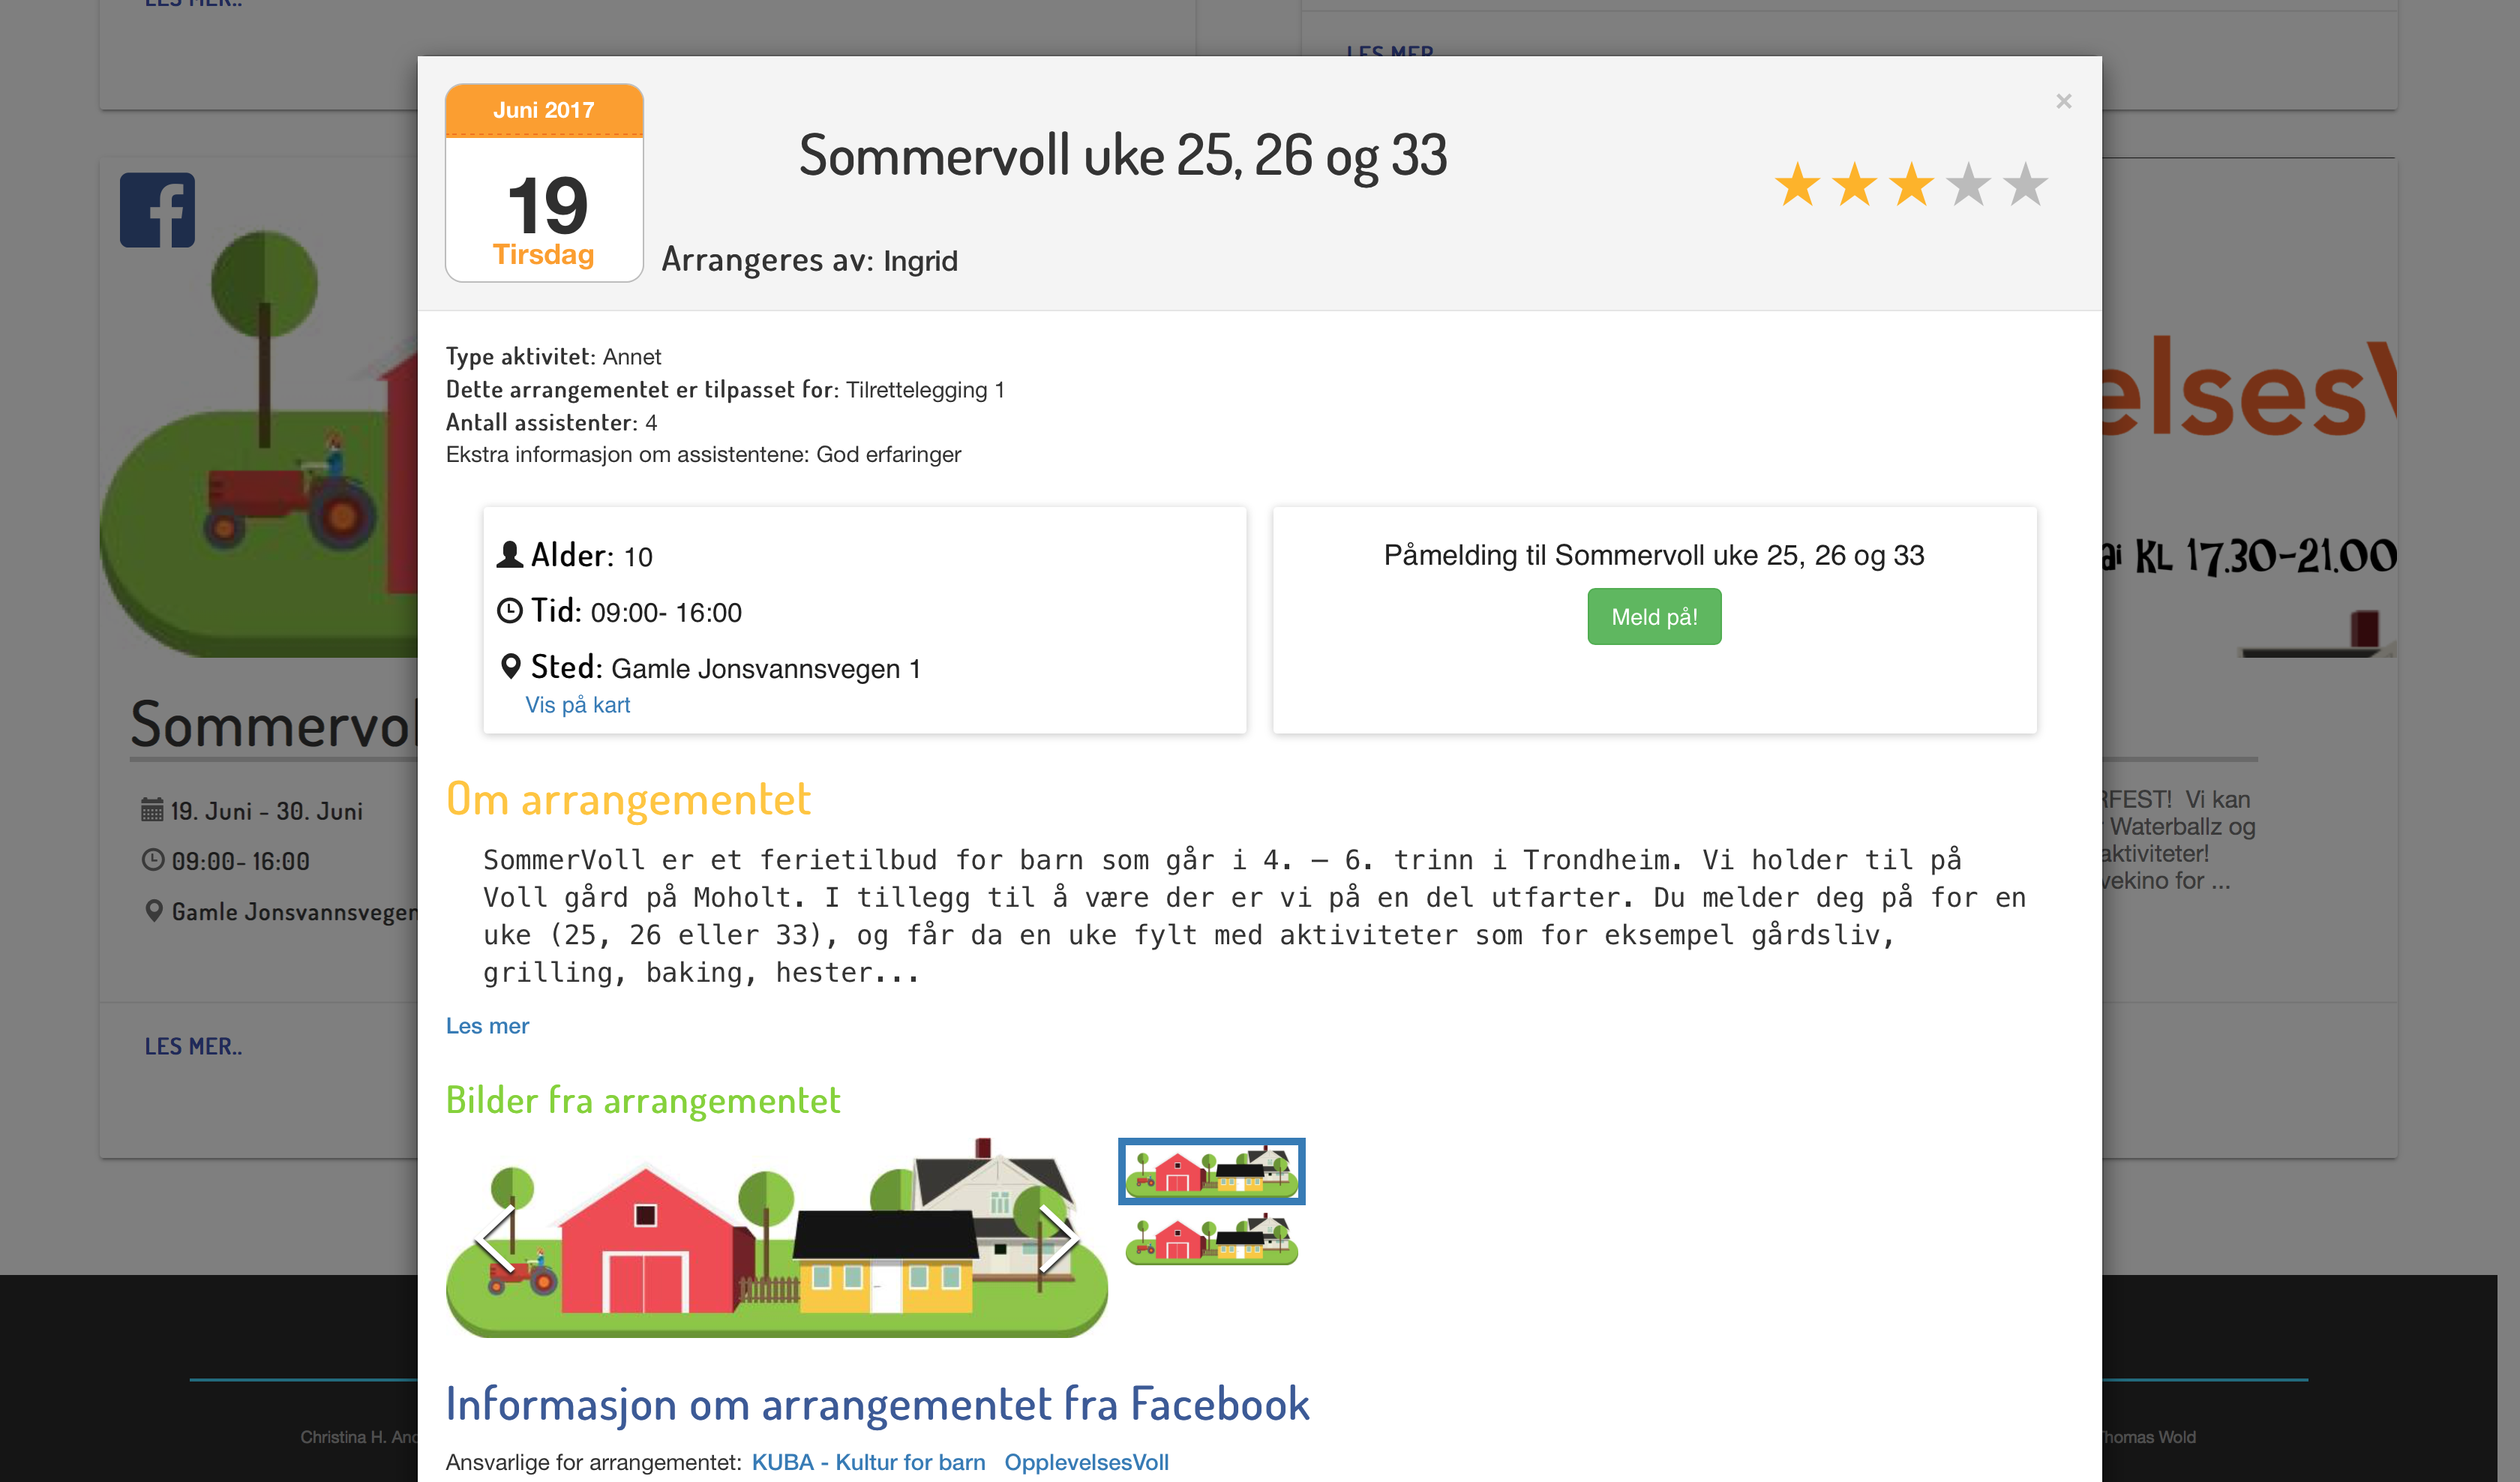
\includegraphics[width=\textwidth]{fig/modal.png}
\caption{User Interface - modal}
\label{Modal}
\end{figure}

\cleardoublepage